\section{Our Existing Software Engineering Framework}

%CUT The recreation of the web application presented the student programmers with the opportunity to learn how to reevaluate the needs of the consumer, while also getting the chance to practice all the skills needed to rebuild an existing application from the ground up inside of a specified time frame. The rebuild process started with the student programmers sitting down and identifying all of the inefficiencies and bugs found in the original web application, from the standpoint of both the user and the programmer. Once all of the major issues were addressed, the next step was to go through several iterations of paper prototyping to redesign the some of the major user interfaces of the web application. The student programmers needed to learn how to consider how users could interact with any given user interface in every possible way. The iterations of paper prototyping also helped the student programmers transition into building the database schema, because paper prototyping allowed them to develop a sense of what data would be necessary to populate the user interfaces. After the conclusion of this step, the student programmers set off in pairs to begin the reconstruction of the original web application. The student programmers learned and followed Agile principles using a modified version of Scrum to carry out their programming duties, with the end goal of creating a working demo of the web application by the end of the summer. At the conclusion of the summer, the student programmers demoed their work to the Labor Office staff and received incredibly positive feedback. The Labor Office staff was relieved to see how the new web application took care of almost all of their needs, and even handled issues they did not realize could be automated and therefore the demo was an overall success. Following the demo, the students went through rounds of design, development, testing, and live demos to ensure the application considered the new feedback. The software is currently very near completion, and should be deployed soon after the submission of this research paper.

Over a six year period, a process was created and refined that informed the current framework, which is designed for employing students as software developers for the purpose of developing applications for an academic institution. Following best practices in lean thinking, the current framework has constantly been evaluated, redesigned, and optimized over the last six years. Thus, the framework presented in this section represents its current state and has been generalized as much as possible, but will certainly change as the needs of the team evolve.

The team of students follow Agile principles \cite{agilemanifesto} using a modified version of Scrum \cite{thescrumguide}. The Scrum methodology dictates that there are three key roles in which all those involved with the development of a software fall under: product owner, Scrum Master, and the development team. The product owner, in relation to the team, is the customer who makes a software request and determines the vision and purpose of the software product. Newly added features, fixed bugs, and completed software must be approved and accepted by the product owner before it is considered complete. The Scrum Master is charged with the responsibility of supporting and facilitating the development team and communicating the needs of the product owner. In our framework, the Scrum Master is typically a full-time employee of the college, though a student could assume this role if they have been on the team a significant number of years and can handle the responsibility of guiding the development of the software. Finally, the development team in this framework consists of undergraduate students who are ``structured and empowered by the organization to organize and manage their own work'' \cite{thescrumguide}. Following Scrum theory provides an iterative, yet incremental approach to cut down on risks and enhance the predictability of the project for the product owner and the development team.

Scrum also prescribes four events in the software engineering process: sprint planning, the sprint, sprint review, and sprint retrospective. These four events are implemented differently in the framework depending on the term.  In the summer, the team follows a more traditional Scrum model with a product backlog and work in progress determined during spring planning, daily Scrum meetings occurring during the sprint, and a Sprint Review and Retrospective happening every two to three weeks before starting the next cycle. In a typical regular term (i.e., a Fall and Spring term consisting of 16 weeks each), the Scrum time-frame is stretched out due to students working only 10 hours per week instead of 40 hours per week. Daily Scrums become weekly, and Sprints take four to six weeks. Because the regular term is significantly less hours worked, we often save new systems and major features for the upcoming summer term, while smaller features and bug fixes happen during the regular term.

This next section will first describe our framework during the summer term, coined the Summer Internship Phase. Then, the following section will describe the framework during the fall and spring terms, coined the Maintenance and Customer Support Phase.

\subsection{The Summer Internship Phase}
Starting in the summer term, students are hired into the SSDT based on a few metrics, including grades in key classes, their ability to work well with others (namely, pair programming \cite{2002PairProgramming}, and the perceived value they will attain from participating in the program (i.e., the best computer science students are not always selected, as they may not benefit as much from the program), to name a few.

A typical summer operates much like an internship, where students are employed for 40 hours per week for 8-10 weeks, resulting in up to 400 hours of software engineering experience. Their expectations mirror an internship in many ways, in that they are expected to be punctual, be productive throughout the day, and regularly report their progress to supervisors. Each summer consists of six to ten students managed by one faculty and two staff (the leadership team). The students work in pairs as they design interfaces and develop code. Very rarely will a student have been explicitly trained on software engineering principles such as Agile methodologies, Model-View-Controller (MVC) or similar frameworks, or large-scale application development, prior to joining the team.

%Contrary to what might seem obvious, the students do not spend a significant amount of time in ``training.'' Instead, we follow a ``just-in-time'' learning principle, where the students are given only as much theory and knowledge about software engineering as is needed to begin the task at hand. For example, one of the first skills students must develop is the ability to work in a version control system, in our case, git. Students are walked through Git basics, such as how to clone the repository, make commits, and issue pull requests, and then they are given their first issue from the issue queue. Their first issue is often selected very intentionally by the supervisors; for example, finding and fixing a typo in a README of one of the repositories. This gives them the confidence to make a change and issue a pull request to the repository owner, without the fear of breaking any system.

A key skill gained by our students very early in the summer internship is the ability to translate customer's needs into usable software (i.e., requirements gathering and design). Students begin by paper prototyping \cite{2003paperPrototype} a design of the application. This design process consists of many iterations of interfaces on paper. Designs are critiqued and modified until there is a group consensus to move forward. This avoids the students spending significant hours writing code that doesn’t match the team’s understanding of the application or the product owner’s needs.

After paper prototyping, the students begin to construct the models that support their prototype. As a group, they participate in a model building session in which they propose the underlying data structures of the application and the relationships between parts of the model. This process provides students with a better understanding of the models when they begin implementing their prototypes, reducing confusion about how data is stored and retrieved.

Having a design in place and an understanding of the data model, the students are ready to begin building the application. Students are first given a virtual machine (VM) to develop on, which mirrors the production environment, but also requiring them to learn some basic Linux commands and usage (again, a new skill for most). Working from a template, pairs of students begin construction from a common git repository with a pre-loaded template.

Throughout the process described above, students meet every morning for a daily Scrum. It is encouraged and expected that students will have plenty of questions early on in the summer internship. In fact, most of the training happens as a result of a student asking a question, since the team does not spend significant time doing formal training for the program.

As the summer progresses, the leadership team begins expecting the students to ask each other for help first. This promotes sharing of knowledge among teams, as pairs begin to solve problems that others have already solved (or those similar), and know some of the pitfalls to avoid. To maintain organization and visibility about what features each team is working on, we leverage Kanban boards, or Work in Progress (WIP) boards \cite{anderson2010kanban}. Applying the Kanban model in tandem with the Scrum framework aids in managing the overall flow of the project.

%CUTThe Kanban model prioritizes three essential principles: visualize what will be done today, reduce the amount of work that is in progress, and properly manage the flow. Kanban encourages continued cooperation and creates an environment that promotes ongoing learning by describing the optimal team workflow. The blending of Kanban and Scrum is also known as Scrumban \cite{ladas2009scrumban}. %Figure \ref{kanban} shows the most recent iteration of our Kanban board (which has changed many times as the team finds ways to improve its usefulness).

%\begin{figure}[h]
% \centering
% 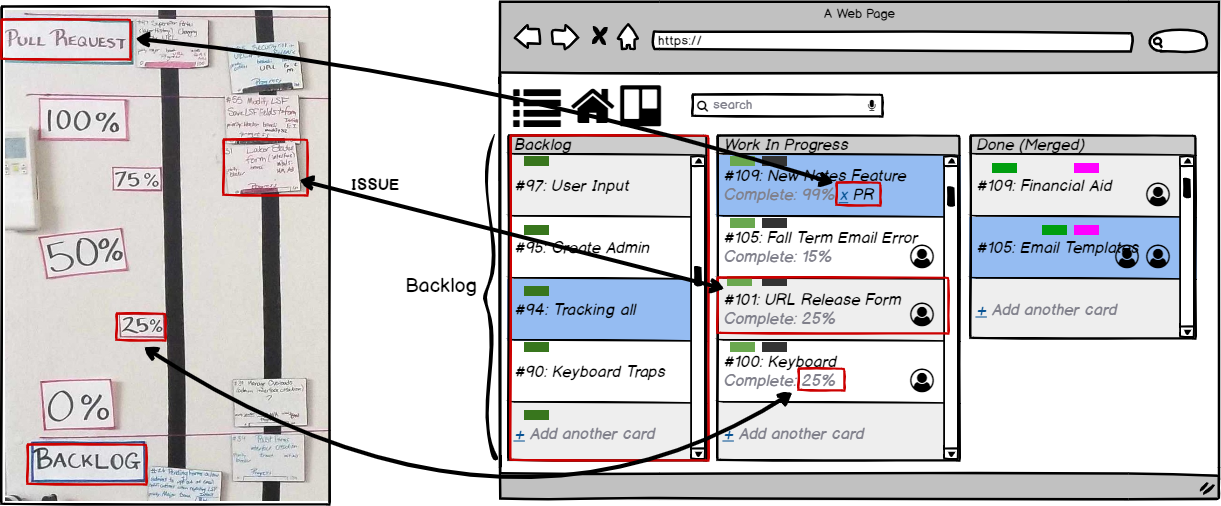
\includegraphics[width=\linewidth]{newTrellomockup2.png}
% \caption{Comparison between physical and virtual Kanban board}
% \label{kanban}
%\end{figure}


%CUTAnother important tactic in promoting the sharing of knowledge involves rotating teams. The team lead and supervising faculty member conduct a meeting a few weeks into the summer term to evaluate each pair's performance. They evaluate each developer's strengths and weaknesses, then redistribute the teams. Typically one developer stays on the interface they were already working on developing, and gain a new partner who is new to the interface. Shuffling the pairs helps students be flexible, learn to collaborate with others, and most importantly, reveals the importance of well-documented code and following coding standards adopted by the team. It also encourages the students to be able to explain their progress, clearly articulate their goals, and know exactly what their code does as they explain it to their new partner.

As interfaces get close to being completed, the pairs begin conducting a usability test \cite{usabilitytesting} to test interactions. The pair will run the usability test first with another team who has not used their interface prior, then the supervisors, and lastly with the product owner to get their final approval of the implementation. Then, the students’ code gets tested for security, coding standards, accessibility guidelines, and bugs before being integrated into the production environment by a member of the leadership team.

%CUT The hosting team provides a set of tasks or scenarios to complete, then observe the user. Usability tests showcase previously unseen faults or unconsidered scenarios in their interfaces thus far. For example, during development, teams will commonly only test the expected use case. The usability test might reveal that there is another set of operations that the user can do which causes a crash. After fixing these new bugs or improvements, they will conduct another usability test, typically with the supervisors as the driver. It is expected that there will be less (but rarely none) new bugs or usability problems to fix. A third (or more) usability test is then conducted with the product owner, to get their final approval of the implementation.

Ideally, by the end of summer, the product is delivered to the customer fully implemented. As this is not always the case, constant communication with the product owner as well as clearly setting expectations very early alleviate issues with surprises about delays in deployment. Any features that aren't completed in the summer term become issues for the team during the regular term, after critical bugs are resolved (more on this in the next section). The team reflects on its progress, what worked well and what did not. Each interface is thoroughly documented of its state and what is left to be done so the next set of developers who take it on will have a good idea of what direction to go in.

\subsection{The Maintenance and Customer Support Phase}
When the Fall term begins, the team shifts from working 40 hours to 10 hours per week, as the students are now also responsible for attending classes and other academic responsibilities. As expected, the productivity of the students shifts dramatically between summer and the regular terms. The framework takes this into consideration. The team shifts its focus to maintaining existing software and responding to customer needs (e.g., bug fixes or small feature requests). Students gain valuable experience of having to maintain their software after deployment, a skill rarely taught in software engineering courses after projects are ``completed'' and delivered to customers.

%CUT Students meet with the supervisors at the beginning of the Fall term to schedule their hours around their courses and other academic responsibilities, with the goal of ensuring no student is working alone for extended periods of time. Students who work alone for too much of their time develop bad coding habits without their code being reviewed frequently, leading to wasted effort as the code they create doesn't make it to the final product. Similarly, students working alone often make poor design and usability choices as they implement, leading to useless software. Lastly, if the student gets stuck on a problem, there is no one there to brainstorm solutions with them. The supervisor, in our case a faculty also teaching courses, isn't as available to assist the students as quickly, meaning they must rely on each other to get unstuck more-so than during the summer. It is crucial that students work with other students to fix bugs and solve problems in order to maintain steady progress in development.

Work duties are mostly determined by the users as they encounter bugs, and the product owner, as they start thinking of new features they want in their software. New issues are added to the issue queue for that application as they are reported. Urgent issues are taken by the first available student. Non-critical issues are discussed in the weekly scrum meeting and added to a team’s work in progress, or left in the issue queue for the next week.

%CUT Customers report bugs or new feature requests via email to the supervisors, who evaluate the priority and difficulty of the issue. The issue is then added to the issue queue for that application. If the issue is urgent (e.g., causing crashes or rendering an interface unusable), the issue is taken by the first student that is available (i.e., the next one to come to work). In some cases, the bug warrants one or more of the supervisors to work on the issue immediately. For non-critical issues, the issue is discussed in the weekly scrum meeting and added to a team's work in progress, or left in the issue queue if it's not considered the most pressing issue for that week.

% Back to the kanban board...
Similar to summer, the Kanban board is instrumental to keeping the team organized and aware of each others' work, particularly since the students' schedules become more spread out. Students check the Kanban wall for new issues, claim them, and keep record of their progress on the wall. This flow helps developers visualize their progress and estimate their time, which is essential given they only have 10 hours per week to work. When the issue is resolved and tested, a pull request is created and reviewed by the supervisors.

%CUTand returned if there are errors or standards not followed. An accepted pull request must pass our guidelines for coding structure, naming conventions, security, and best practices. The supervisors are responsible for the last mile; integrating the feature into the production environment. Sometimes bugs are found during integration, which are pushed back down into the repository, requiring all developers to pull in these changes (as well as the new feature itself) to synchronize the everyone's local environments.

\section{Shifting Process in Response to COVID-19}
In March 2020, the World Health Organization (WHO) officially classified the coronavirus, COVID-19, outbreak as a pandemic \cite{covid}. Following this declaration, our institution made the decision to close its campus within the week of the WHO’s announcement, one of the earliest campuses to shut down due to the COVID-19 crisis.

Following this closure, the SSDT was ended for the remainder of the Spring 2020 term. Only the leadership team continued to work on the software systems in our last sprint. A few changes were required in our existing systems to support the shutdown itself. For example, every course needed an updated syllabus outlining how classes would change for the remaining eight weeks, which were quickly shifting to emergency online teaching. One of our software systems was currently being used to collect syllabi during regular terms; our team quickly modified the system to support an addition, ``odd'' term, where faculty could quickly and easily upload syllabi.

The SSDT team is also responsible for the creation and maintenance of the software used for planning courses each term. Our system allows all department chairs to construct a pre-plan schedule of classes each term before they are inserted into the official catalog. This allows multiple departments to collaborate on schedules, ensuring courses required for majors but outside a major aren't at conflicting times. Our software will be handling a new, unknown schedule for the fall, which our team will have to test before it can go live to the rest of the community. Our students will be doing a significant amount of this work in the coming weeks, once an official schedule is released by the institution.

The SSDT team was approved to allow students to work in the work-study program for the remainder of the summer, only the work had to be remote-only; no in-person meetings. The team had to quickly adapt its model to this new work environment. One of the many considerations that had to be acknowledged during this process is that some students were now dealing with outside distractions that did not exist when working in our space, including moving back in with their families, balancing parenting and other duties, and unreliable Internet and technology at home.

The leadership team prepared by reprioritizing all of the remaining issues in the queue. The leadership team then did a thorough walkthrough of the current application to identify new issues that were created when the students left campus, as some work was unfinished and left in a poor state due to the students leaving in a hurry. The final and most important step was deciding which tools the team would use that would most closely resemble the workflow that existed while on-campus.  Ultimately, the leadership team identified four tools that were key to facilitating student success in a remote SSDT environment: 1) a digital version of the Kanban board for organizing tasks; 2) a communication platform to facilitate online meetings and design/code reviews; 3) a wireframing tool for creating low fidelity prototypes for demonstrating user flow, user interfaces, and user experience testing, which was replacing our paper prototyping process; and 4) a collaborative code editor where two or more programmers could write code and see changes in real-time, modeling pair programming. The next section details how these tools were leveraged by the team.

\subsection{New Tools and Processes}
Above all else, constant and consistent communication between the students and the leadership team was of the utmost importance. Having good visibility on what everyone was working on would be the first step in ensuring progress was maintained. An online Kanban board was obtained to digitize the physical board in our space. Figure~\ref{fig:digitalkanban} shows the old and new versions of the Kanban board, and also indicates related objects on each.

\begin{figure}[h]
 \centering
 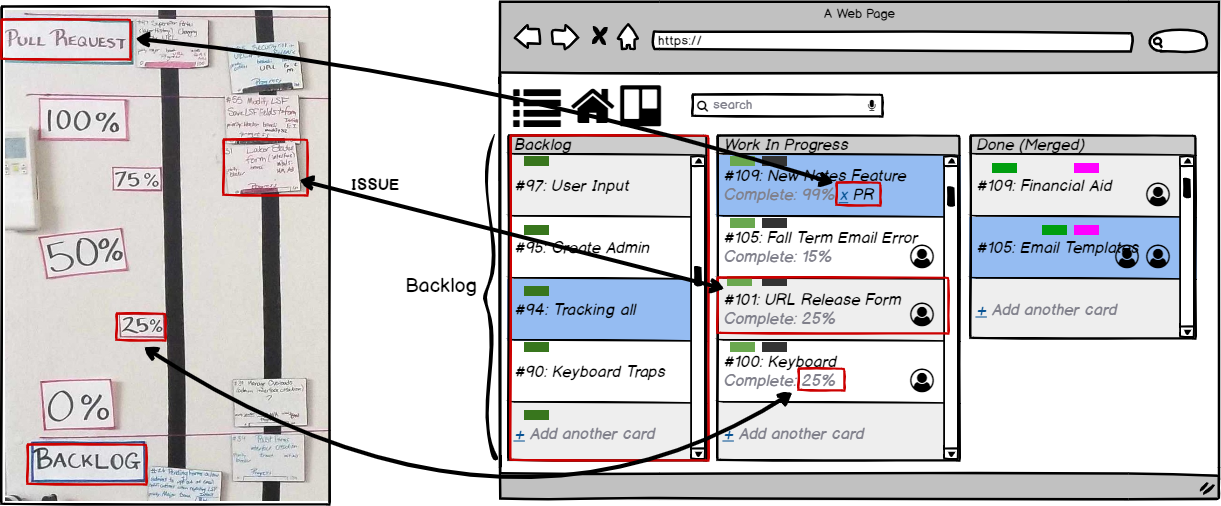
\includegraphics[width=\linewidth]{newTrellomockup2.png}
 \caption{Comparison between physical and virtual Kanban board}
 \label{fig:digitalkanban}
\end{figure}

The SSDT already utilized a communication platform for much of its online communication, so it was decided to continue with a more significant reliance on this tool. The student programmers were given a consistent structure for reporting progress, following a ``Did, Doing, Stuck'' (DDS) structure, where the students would explain what they did the previous day, what they will be doing this work day, and if they are stuck on anything. The leadership team would check these updates daily to monitor progress and ensure students are not stuck for an extended amount of time, closely mirroring our process before the crisis. The communication platform also offered video calling capabilities, allowing the team to continue doing Scrum meetings as they did the in previous summers, just through video conferencing. Video calls also allowed the faculty member to provide ``just-in-time'' training to the newer students of the team, using screen-sharing to simulate whiteboards and share presentations.

Given the situation, students were not able to collaborate in-person to design a paper prototype, so an online collaborative wireframing tool was procured to create mockups of the new interface they were designing. The wireframing tool proved to be about as effective as paper prototyping, because it allowed designs to be responsive and perform like actual webpages (e.g., demonstrating ``on click" events). This change in our development process ensured that the team did not stray from our prescribed software process and also introduced a tool that provides an efficient way to prototype interfaces.

Pair programming was an important element to the learning experience in the SSDT program. Students were required to work in pairs at a single workstation, alternating between driving and navigating. This aspect of software engineering was particularly important to the leadership team, as it teaches the students the importance of working with others, being willing to ask questions, and thinking about the structure of code while it's being developed. The programmers used the communication platform to facilitating communication, remaining on a video call during the entire time that they were working in order to replicate the conversations that they would have if they were next to each other. However, coding together when not looking at the same terminal is highly ineffective. So, a plugin was added to their IDEs that allowed them to share their code with their partner and see each other's edits in real-time. The leadership team could also use this plugin to perform code reviews with the student teams.

Anecdotal evidence suggests that the students are feeling productive, efficient, and are still learning a lot from the experience. The leadership team regularly asks the students in the morning scrum meetings to provide feedback to them about how to improve this process for them. They are mostly indicating they simply need practice and time to develop the skills needed, which is largely in line with what is expected of them when in person.
